%%%%%%%%%%%%%%%%%%%%%%%%%%%%%%%%%%%%%%%%%%%%%%%%%%%%%%%%%%%%%%%%%%%%%%%%
% Plantilla Ejemplos de Uso
% Escuela Politécnica Superior de la Universidad de Alicante
% Realizado por: Jose Manuel Requena Plens
% Contacto: info@jmrplens.com / Telegram:@jmrplens
%%%%%%%%%%%%%%%%%%%%%%%%%%%%%%%%%%%%%%%%%%%%%%%%%%%%%%%%%%%%%%%%%%%%%%%%
\section{Ejemplos de uso de la plantilla}

Para citar la bibliografía tal como se define en IEEE usar \cite{ruiz2016guia}. Por ejemplo:

\begin{lstlisting}[style=Latex-color]
Basado en estudio recientes \cite{Aguilar2013} se puede comprobar que... y 
complementando este hecho por lo desarrollado previamente \cite{LopezJimenez2013} 
podemos afirmar que..
\end{lstlisting}

Para citar la bibliografía tal como se define en el sistema APA (en esta web se indica como debe aparecer en el texto la cita: \url{http://guides.libraries.psu.edu/apaquickguide/intext}) se debe realizar con alguno de los comandos mostrados a continuación:

\begin{lstlisting}[style=Latex-color]
Esto es una cita estándar: \citet{Shaw1996}, que también puedes mostrar con paréntesis así: \citep{Shaw1996}. También se puede realizar una cita indicando a qué parte te refieres \citep[ver][Cap. 2]{Shaw1996} o \citep[Cap. 2]{Shaw1996} o \citep[ver][]{Shaw1996}. 

También puedes mostrar todos los autores cuando hay más de 2 autores añadiendo un asterisco después del comando como: \citet*{Akyildiz2005}, sin el asterisco quedaría así: \citet{Akyildiz2005}.

O puedes citar dos o más fuentes al mismo tiempo: \citep{Barkan1995,Leighton2012}

\end{lstlisting}
Y \LaTeX~genera lo siguiente:
\\
\par Esto es una cita estándar: \citet{Shaw1996}, que también puedes mostrar con paréntesis así: \citep{Shaw1996}. También se puede realizar una cita indicando a qué parte te refieres \citep[ver][Cap. 2]{Shaw1996} o \citep[Cap. 2]{Shaw1996} o \citep[ver][]{Shaw1996}. 
\\
\par También puedes mostrar todos los autores cuando hay más de 2 autores añadiendo un asterisco después del comando como: \citet*{Akyildiz2005}, sin el asterisco quedaría así: \citet{Akyildiz2005}.
\\
\par O puedes citar dos o más fuentes al mismo tiempo: \citep{Barkan1995,Leighton2012}


\section{Notas a pie de página}

Para introducir notas a pie de página se debe escribir lo siguiente:

\begin{lstlisting}[style=Latex-color]
	La plantilla necesita el motor XeLaTeX \footnote{Para más información sobre XeLaTeX visita \url{https://es.sharelatex.com/learn/XeLaTeX}} (el más recomendable actualmente), por lo que si el programa que utilizas compila la plantilla con el motor pdfLaTeX \footnote{También puedes buscar más información en internet} (el más habitual pero menos potente) debes cambiarlo por XeLaTeX en las opciones del programa. Si no sabes como hacerlo busca en el manual del programa o en google.
\end{lstlisting}

\LaTeX~genera lo siguiente (observa las notas a pie de página):
\\
\par La plantilla necesita el motor XeLaTeX\footnote{Para más información sobre XeLaTeX visita \url{https://es.sharelatex.com/learn/XeLaTeX}} (el más recomendable actualmente), por lo que si el programa que utilizas compila la plantilla con el motor pdfLaTeX\footnote{También puedes buscar más información en internet} (el más habitual pero menos potente) debes cambiarlo por XeLaTeX en las opciones del programa. Si no sabes como hacerlo busca en el manual del programa o en google.
\section{Estilos de texto}

A continuación se muestran ejemplos de distintos estilos de texto:

\begin{itemize}
	\item \textbackslash textit\{Cursiva\} $\rightarrow$ \textit{Cursiva}
	\item \textbackslash emph\{Cursiva 2\} $\rightarrow$ \emph{Cursiva 2}
	\item \textbackslash textbf\{Negrita\} $\rightarrow$ \textbf{Negrita}
	\item \textbackslash texttt\{Monoespacio\} $\rightarrow$ \texttt{Monoespacio}
	\item \textbackslash textsc\{Mayúsculas capitales\} $\rightarrow$ \textsc{Mayúsculas capitales}
	\item \textbackslash uppercase\{Todo mayúsculas\} $\rightarrow$ \uppercase{Todo mayúsculas} 
\end{itemize}

 \section{Acrónimos}
 Ahora vamos a ver cómo se ponen los acrónimos.
 
 La norma dice que la primera vez que aparece un acrónimo debe ponerse su fórmula completa, es decir lo que significa, al lado del acrónimo. Después de ello, podemos usar sólo el acrónimo salvo cuando consideremos que debemos volver a usar la fórmula completa por alguna razón de legibilidad.
 
 ¿Cómo llevar la cuenta de cuándo es la primera vez que ponemos el acrónimo? si hacemos cambios en el doc es fácil que perdamos esa información así que lo mejor es que sea el propio \LaTeX~el que lleve esa cuenta. Para ello tenemos que hacer dos cosas:
 \begin{description}
 \item[Primero:] creamos la entrada del acrónimo en el fichero acronimos.tex. Revisa los comentarios de su cabecera para saber cómo crear esa entrada. Básicamente lo que hacemos allí es poner la ``fórmula corta'' y la ``fórmula larga'' del acrónimo es decir, el propio acrónimo y su significado
 \item[Segundo:] escribimos en el texto el acrónimo SIEMPRE diciendo que es un acrónimo y el tipo de fórmula que queremos usar. Por ejemplo, si siempre que queremos hacer referencia al IEEE escribimos \begin{lstlisting}[style=Latex-color]
 \gls{ieee}
 \end{lstlisting}  se consigue que la primera vez que aparezca el acrónimo ponga las fórmulas larga y corta y en las siguientes ocasiones sólo aparecerá la corta.
 \end{description}
 
 Aquí va un ejemplo:
 
 Si escribimos:
 
\begin{lstlisting}[style=Latex-color]
 El \gls{ieee} es una institución muy importante en el mundo de la
 ingeniería.  El \gls{ieee} lleva marcando normas y protocolos desde
 hace mucho tiempo.  Pero el \gls{ieee} no está solo en esta tarea. 
 Además del \gls{ieee} hay muchas otras instituciones para ello.  \end{lstlisting}
 
 Obtendremos: 
 
El \gls{ieee} es una institución muy importante en el mundo de la
 ingeniería.  El \gls{ieee} lleva marcando normas y protocolos desde
 hace mucho tiempo.  Pero el \gls{ieee} no está solo en esta tarea. 
 Además del \gls{ieee} hay muchas otras instituciones para ello.

\section{Listas}
Hacer una lista es simple en \LaTeX. Para ello has de crear un entorno (así se llama) itemize con
\begin{lstlisting}[style=Latex-color]
\begin{itemize}
...
\end{itemize}
\end{lstlisting}
Y dentro de esa estructura, añadir cada elemento de la lista precedido de 
\begin{lstlisting}[style=Latex-color]
\item primer ítem de lista
\item segundo ítem de lista
...
\item ultimo ítem de lista
\end{lstlisting}

Es importante que revises este texto tal como aparece en la plantilla y relaciones el aspecto que tiene el PDF final con cómo está escrito el documento \LaTeX.
\vspace{1em}
\noindent\hrule
\vspace{1em}

Aquí va una lista con subtérminos:
\begin{lstlisting}[style=Latex-color]
	\begin{itemize}
    \item Ingeniería Informática.
    \item Ingeniería Sonido e Imagen en Telecomunicación.
    \item Ingeniería Multimedia.
         \subitem Mención: Creación y ocio digital.
         \subitem Mención: Gestión de Contenidos.
	\end{itemize}
\end{lstlisting}

El resultado es el siguiente:
\begin{itemize}
    \item Ingeniería Informática.
    \item Ingeniería Sonido e Imagen en Telecomunicación.
    \item Ingeniería Multimedia.
         \subitem Mención: Creación y ocio digital.
         \subitem Mención: Gestión de Contenidos.
\end{itemize}
\vspace{1em}
\noindent\hrule
\vspace{1em}
Aquí va una lista con subtérminos pero numerada:
\begin{lstlisting}[style=Latex-color]
\begin{enumerate}
    \item Ingeniería Informática.
    \item Ingeniería Sonido e Imagen en Telecomunicación.
    \item Ingeniería Multimedia.
    \begin{enumerate}
         \item Mención: Creación y ocio digital.
         \item Mención: Gestión de Contenidos.
   	\end{enumerate}
\end{enumerate}
\end{lstlisting}

El resultado es el siguiente:
\begin{enumerate}
    \item Ingeniería Informática.
    \item Ingeniería Sonido e Imagen en Telecomunicación.
    \item Ingeniería Multimedia.
    \begin{enumerate}
         \item Mención: Creación y ocio digital.
         \item Mención: Gestión de Contenidos.
   	\end{enumerate}
\end{enumerate}

\section{Listas de definición}
 
 Puedes realizar una lista de conceptos con su definición del siguiente modo:
 
\begin{lstlisting}[style=Latex-color]
\begin{description} % Inicio de la lista
 	\item[MAPP XT:] Programa desarrollado por \textit{Meyer Sound} para el diseño y ajuste de sistemas formados por altavoces de su marca.
  	\begin{description} % Realiza una lista dentro de la lista
  		\item[Ventajas:]~ 
  		El programa permite realizar múltiples ajustes tal como se podría realizar en la realidad con un procesador real.
  	
  		Permite analizar la fase recibida en cualquier punto y compararla con otras mediciones.
  	
  		Dispone de varios tipos de filtros, inversiones de fase, etc.
  		\item[Inconvenientes:]~ 
  		No existe una lista global de los altavoces ubicados en el plano, por lo tanto solo se pueden editar seleccionándolos sobre el plano.
  	
  		Sólo permite diseñar en 2 dimensiones, principalmente sobre la vista lateral ya que los array de altavoces no permite voltearlos.
  	\end{description}
\end{description}
\end{lstlisting}

 Y \LaTeX~genera lo siguiente:
 
\begin{description} % Inicio de la lista
 	\item[MAPP XT:] Programa desarrollado por \textit{Meyer Sound} para el diseño y ajuste de sistemas formados por altavoces de su marca.
  	\begin{description} % Realiza una lista dentro de la lista
  		\item[Ventajas:]~ 
  		El programa permite realizar múltiples ajustes tal como se podría realizar en la realidad con un procesador real.
  	
  		Permite analizar la fase recibida en cualquier punto y compararla con otras mediciones.
  	
  		Dispone de varios tipos de filtros, inversiones de fase, etc.
  		\item[Inconvenientes:]~ 
  		No existe una lista global de los altavoces ubicados en el plano, por lo tanto solo se pueden editar seleccionándolos sobre el plano.
  	
  		Sólo permite diseñar en 2 dimensiones, principalmente sobre la vista lateral ya que los array de altavoces no permite voltearlos.
  	\end{description}
\end{description}

\section{Inserción de código}
A veces tendrás que insertar algún pedazo de código fuente para explicar algo relacionado con él. No sustituyas explicaciones con códigos enormes. Si pones algo de código en tu TFG que sea para demostrar algo o explicar alguna solución.

\LaTeX~te ayuda a escribir código de manera que su presentación tenga las marcas y tabulaciones propias de este tipo de texto. Para ello, debes poner el código que escribas DENTRO de un entorno  que se llama ``listings''.  La plantilla ya tiene una serie de instrucciones para incluir el paquete ``listings'' y añadirle algunos modificadores por lo que no tienes que incluirlo tú. Simplemente, mete tu código en el entorno ``lstlisting'' y ya está. Puedes indicar el lenguaje en el que está escrito el código y así \LaTeX~lo mostrará mejor. 
\\
\par En el archivo \textit{estiloscodigoprogramacion.tex} están definidos algunos lenguajes para mostrarlos con un diseño concreto, se pueden modificar para cambiar el coloreado del código, qué términos se ponen en negrita, etc.
Si se quiere profundizar más en la función ``listings'' se puede consultar su manual en \url{http://osl.ugr.es/CTAN/macros/latex/contrib/listings/listings.pdf}, aunque hay mucha información en foros y blog's que es más fácil de comprender.

\par Veamos un ejemplo en la figura \ref{C_code}:

\begin{lstlisting}[style=Latex-color]
\begin{lstlisting}[style=C, caption={ejemplo código C},label=C_code]
	#include <stdio.h>
	int main(int argc, char* argv[]) {
  	puts("Hola mundo!");
	}
\ end{lstlisting}	
\end{lstlisting}

El resultado será:
\begin{lstlisting}[style=C, caption={ejemplo código C},label=C_code]
#include <stdio.h>
// Comentario
int main(int argc, char* argv[]) {
  puts("Hola mundo!");
}
\end{lstlisting}
\vspace{1em}
\noindent\hrule
\vspace{1em}
Si lo quieres en color, está definido el estilo C-color en el archivo \textit{estiloscodigoprogramacion.tex}, con algunos parámetros para mejorar la visualización:
\begin{lstlisting}[style=Latex-color]
\begin{lstlisting}[style=C-color, caption={ejemplo código C en color},label=C_code-color]
#include <stdio.h>
// Comentario
int main(int argc, char* argv[]) {
  puts("Hola mundo!");
}
\ end{lstlisting}
\end{lstlisting}
\begin{lstlisting}[style=C-color, caption={ejemplo código C en color},label=C_code-color]
	#include <stdio.h>
	// Comentario
	int main(int argc, char* argv[]) {
  	puts("Hola mundo!");
	}
\end{lstlisting}
\vspace{1em}
\noindent\hrule
\vspace{1em}
Por supuesto, puedes mejorar esta presentación utilizando más modificadores. En la sección \ref{usos} se indican algunos detalles.

Otro ejemplo, ahora para mostrar código PHP, sería escribir en tu fichero \LaTeX~lo siguiente:
\begin{lstlisting}[style=Latex-color,numbers=none]
 \begin{lstlisting}[style=PHP, caption={ejemplo código PHP},label=PHP_code]
 /* 
Ejemplo de código en PHP para escribir tu primer programa en este lenguaje
Copia este código en tu ordenador y ejecútalo
*/
<html>
  <head>
    <title>Prueba de PHP</title>
  </head>
  <body>
    <?php echo '<p>Hola Mundo</p>'; ?> //esto lo escribe TODO el mundo
  </body>
</html>
 \ end{lstlisting}
\end{lstlisting}
 
 y el resultado es el siguiente:
 
 \begin{lstlisting}[style=PHP, caption={ejemplo código PHP},label=PHP_code,firstnumber=100]
/* 
Ejemplo de código en PHP para escribir tu primer programa en este lenguaje. Copia este código en tu ordenador y ejecútalo
*/
 <html>
  <head>
    <title>Prueba de PHP</title>
  </head>
  <body>
    <?php echo '<p>Hola Mundo</p>'; ?> //esto lo escribe TODO el mundo
  </body>
</html>
 \end{lstlisting}
 \vspace{1em}
\noindent\hrule
\vspace{1em}
 O también en color: 
 \begin{lstlisting}[style=PHP-color, caption={ejemplo código PHP},label=PHP_code2]
/* 
Ejemplo de código en PHP para escribir tu primer programa en este lenguaje. Copia este código en tu ordenador y ejecútalo
*/
 <html>
  <head>
    <title>Prueba de PHP</title>
  </head>
  <body>
    <?php echo '<p>Hola Mundo</p>'; ?> //esto lo escribe TODO el mundo
  </body>
</html>
 \end{lstlisting}
 
 Observa cómo \LaTeX~ha puesto los comentarios en gris y ajustado el código para que se muestre más claro.
\vspace{1em}
\noindent\hrule
\vspace{1em}
 A continuación se muestran otros ejemplos:
 \begin{lstlisting}[style=Matlab-color, caption={ejemplo código Matlab en color},label=Matlab_code]
%% Code sections are highlighted.
% System command are supported...
!touch testFile.txt
A = [1, 2, 3;... %... as is line continuation.
     4, 5, 6];
fid = fopen('testFile.text', 'w');
for k=1:10
  fprintf(fid, '%6.2f \n', k)
end
x=1; %% this is just a comment, not the start of a section
% Context-sensitive keywords get highlighted correctly...
p = properties(person); %(here, properties is a function)
x = linspace(0,1,101);
y = x(end:-1:1);
% ... even in nonsensical code.
]end()()(((end while {    end    )end ))))end (end
%{
    block comments are supported
%} even
runaway block comments are
\end{lstlisting}

\begin{lstlisting}[style=Matlab, caption={ejemplo código Matlab en blanco y negro},label=Matlab_codebn]
%% Code sections are highlighted.
% System command are supported...
!touch testFile.txt
A = [1, 2, 3;... %... as is line continuation.
     4, 5, 6];
fid = fopen('testFile.text', 'w');
for k=1:10
  fprintf(fid, '%6.2f \n', k)
end
x=1; %% this is just a comment, not the start of a section
% Context-sensitive keywords get highlighted correctly...
p = properties(person); %(here, properties is a function)
x = linspace(0,1,101);
y = x(end:-1:1);
% ... even in nonsensical code.
]end()()(((end while {    end    )end ))))end (end
%{
    block comments are supported
%} even
runaway block comments are
\end{lstlisting}
\newpage
\begin{lstlisting}[style=Python-color, caption={ejemplo código Python en color}]
class Example (object):
    def __init__ (self, account, password):
        """e.g. account  = 'bob@example.com/test'
                password = 'bigbob'
        """

        reg = telepathy.client.ManagerRegistry()
        reg.LoadManagers()

        # get the gabble Connection Manager
        self.cm = cm = reg.GetManager('gabble')

        # get the parameters required to make a Jabber connection
        # begin ex.basics.dbus.language-bindings.python.methods.call
        cm[CONNECTION_MANAGER].RequestConnection('jabber',
            {
                'account':  account,
                'password': password,
            },
            reply_handler = self.request_connection_cb,
            error_handler = self.error_cb)
        # end ex.basics.dbus.language-bindings.python.methods.call
\end{lstlisting}

\begin{lstlisting}[style=Python, caption={ejemplo código Python en blanco y negro}]
class Example (object):
    def __init__ (self, account, password):
        """e.g. account  = 'bob@example.com/test'
                password = 'bigbob'
        """

        reg = telepathy.client.ManagerRegistry()
        reg.LoadManagers()

        # get the gabble Connection Manager
        self.cm = cm = reg.GetManager('gabble')

        # get the parameters required to make a Jabber connection
        # begin ex.basics.dbus.language-bindings.python.methods.call
        cm[CONNECTION_MANAGER].RequestConnection('jabber',
            {
                'account':  account,
                'password': password,
            },
            reply_handler = self.request_connection_cb,
            error_handler = self.error_cb)
        # end ex.basics.dbus.language-bindings.python.methods.call
\end{lstlisting}

\section{Usos y personalización}
\label{usos}

El texto que acompaña al código puedes incluirlo o no, también puedes decidir si el texto va numerado o no. A continuación se muestra como:
\begin{lstlisting}[style=Latex-color]
	% Con esta línea el código no tendrá título
	\begin{lstlisting}[style=Python]
		micodigo
	\ end{lstlisting}
\end{lstlisting}

\begin{lstlisting}[style=Python]
	micodigo
\end{lstlisting}
\vspace{1em}
\noindent\hrule
\vspace{1em}
\begin{lstlisting}[style=Latex-color]
	% Con esta línea el código tendrá el título abajo
	\begin{lstlisting}[style=Python, caption={Ejemplo de título abajo},captionpos=b]
		micodigo
	\ end{lstlisting}
\end{lstlisting}

\begin{lstlisting}[style=Python,caption={Ejemplo de título abajo},captionpos=b]
	micodigo
\end{lstlisting}
\vspace{1em}
\noindent\hrule
\vspace{1em}
\begin{lstlisting}[style=Latex-color]
	% Con esta línea el código tendrá título no numerado
	\begin{lstlisting}[style=Python, title={Ejemplo de título no numerado}]
		micodigo
	\ end{lstlisting}
\end{lstlisting}

\begin{lstlisting}[style=Python,title={Ejemplo de título no numerado}]
	micodigo
\end{lstlisting}
\vspace{1em}
\noindent\hrule
\vspace{1em}
\begin{lstlisting}[style=Latex-color]
	% Con esta línea el código no tendrá las líneas numeradas
\begin{lstlisting}[style=Python,numbers=none, title={Ejemplo de código sin número de líneas}]
	micodigo
	sin
	número
	de
	líneas
\ end{lstlisting}
\end{lstlisting}

\begin{lstlisting}[style=Python,numbers=none,title={Ejemplo de código sin número de líneas}]
		micodigo
		sin
		número
		de
		líneas
\end{lstlisting}

\section{Importar archivos fuente}

Existe la posibilidad de importar un archivo de código en lugar de copiar su contenido y pegarlo en \LaTeX.

Para realizarlo debes escribir:

\begin{lstlisting}[style=Latex-color]
\lstinputlisting[style=C++-color,caption={Archivo C++ importado}]{archivos/ejemplos/holamundo.cpp}	
\end{lstlisting}

Y se importará con el formato establecido entre los '[ ]':
\newpage
\lstinputlisting[style=C++-color,caption={Archivo C++ importado}]{archivos/ejemplos/holamundo.cpp}

A continuación se muestran otros ejemplos

\begin{lstlisting}[style=Latex-color]
\lstinputlisting[style=Python-color,caption={Archivo Py importado},label=importado_py]{archivos/ejemplos/holamundo.py}	
\end{lstlisting}

\lstinputlisting[style=Python-color,caption={Archivo Py importado},label=importado_py2]{archivos/ejemplos/holamundo.py}	

\begin{lstlisting}[style=Latex-color]
\lstinputlisting[style=Matlab-color,caption={Archivo Matlab importado},label=importado_m]{archivos/ejemplos/holamundo.m}	
\end{lstlisting}

\lstinputlisting[style=Matlab-color,caption={Archivo Matlab importado},label=importado_m]{archivos/ejemplos/holamundo.m}

\section{Diagramas}
Gracias al paquete \textit{Tikz} se pueden incluir multitud de medios gráficos, diagramas, capas sobre imágenes, etc.
Existen múltiples formas de realizarlo, para ello es recomendable consultar la guía de iniciación disponible aquí: \url{http://cremeronline.com/LaTeX/minimaltikz.pdf} y también el manual completo disponible aquí: \url{http://osl.ugr.es/CTAN/graphics/pgf/base/doc/pgfmanual.pdf}.
\\
\par A continuación se muestran algunos ejemplos. Revisa el archivo .tex para ver cómo se utilizan.
\\
\par Imagen a la que se le ha añadido cuadros y texto desde latex:
\begin{figure}[ht]
\centering	
\resizebox{0.6\textwidth}{!}{%
\begin{tikzpicture}[x=39, y=47]%X,Y -> Corrección de coordenadas, según tamaño y posición de la imagen
    \node[anchor=south west,inner sep=0] (image) at (0,0) {\includegraphics[width=0.9\textwidth]{archivos/mapadia}};
    % Imprimir coordenadas
    \begin{scope}[x={(image.south east)},y={(image.north west)}]
        \draw[help lines,xstep=.1,ystep=.1] (0,0) grid (1,1);
        \foreach \x in {0,1,...,9} { \node [anchor=north] at (\x/10,0) {\x}; }
        \foreach \y in {0,1,...,9} { \node [anchor=east] at (0,\y/10) {\y}; }
    \end{scope}
    % Residencias 1
    \draw[Caja1] (6.8,2) rectangle (8.3,4.5);
    \node[Texto2] at (6.8,2) {\textbf{Residencias 1}};
    % Residencias 2
    \draw[Caja1] (1,0.6) rectangle (7.6,1.8);
    \node[Texto2] at (1,0.6) {\textbf{Residencias 2}};
    % Residencias 3
    \draw[Caja1,rotate around={-45:(2.6,3.6)}] (2.6,3.6) ellipse (1cm and 3.1cm);
    \node[Texto2] at (1.2,2.1) {\textbf{Residencias 3}};
    % Hospital
    \draw[Caja1] (1,6) rectangle (3,7);
    \node[Texto2] at (1,6) {\textbf{Hospital}};
    % Colegio
    \draw[Caja1] (2.3,8.5) rectangle (3.9,9.5);
    \node[Texto2] at (2.3,8.5) {\textbf{Colegio}};
    % Numeros de edificios
    \node[Texto3,font=\tiny] at (7.5,4) {\textbf{1}};
    \node[Texto3,font=\tiny] at (7.9,2.9) {\textbf{2}};
    \node[Texto3,font=\tiny] at (7.7,2.3) {\textbf{3}};
    \node[Texto3,font=\tiny] at (7.2,1.2) {\textbf{4}};
    \node[Texto3,font=\tiny] at (6.2,1.2) {\textbf{5}};
    \node[Texto3,font=\tiny] at (4.9,1.2) {\textbf{6}};
    \node[Texto3,font=\tiny] at (3.6,1.2) {\textbf{7}};
    \node[Texto3,font=\tiny] at (2.4,1.2) {\textbf{8}};
    \node[Texto3,font=\tiny] at (1.5,1.7) {\textbf{9}};
    \node[Texto3,font=\tiny] at (1.5,2.5) {\textbf{10}};
    \node[Texto3,font=\tiny] at (1.5,3) {\textbf{11}};
    \node[Texto3,font=\tiny] at (1.8,3.4) {\textbf{12}};
    \node[Texto3,font=\tiny] at (2.2,3.8) {\textbf{13}};
    \node[Texto3,font=\tiny] at (2.5,4.2) {\textbf{14}};
    \node[Texto3,font=\tiny] at (3,4.5) {\textbf{15}};
    \node[Texto3,font=\tiny] at (3.4,4.8) {\textbf{16}};
    \node[Texto3,font=\tiny] at (4,4.8) {\textbf{17}};
    % Nombres de carreteras
    \node[Texto3] at (9.2,7) {\textbf{A-7}};
    \node[Texto3] at (9,1.8) {\textbf{N-1}};
    \node[Texto3] at (4,8) {\textbf{N-2}};
\end{tikzpicture}
}
\end{figure}

En muchas ocasiones es necesario realizar un diagrama de bloques, más abajo se muestra un ejemplo de ello. En la red hay multitud de ejemplos que pueden ser fácilmente modificables para un fin concreto, como por ejemplo en esta web: \url{http://www.texample.net/tikz/examples/tag/block-diagrams/}.
\begin{figure}[ht]
\centering 
\begin{tikzpicture}[node distance=2cm, auto]
	% Cuadros
	\node (pc) [rectvioleta,text width=3cm] {Ordenador{\\}\small{Software: ARTA} \par};
	\node (sound) [rectamarillo, below of=pc, text width=4cm] {Tarjeta de sonido {\\}Tascam US-144MKII \par};
	\node (nexus) [rectverde, right of=sound,xshift=6cm, text width=8cm] { Amplificador/Adaptador de impedancia{\\}DIY\par };
	\node (acel) [rectnaranja, below of=nexus,text width=3cm,xshift=0cm]{\small Acelerómetro {\\}Brüel {\&} Kjær TYPE 4514B-002 \par};
	\node (micro) [rectnaranja, below of=sound,text width=3cm,xshift=0cm]{\small Micrófono {\\}Behringer ECM8000 \par};
	\node (excit) [rectnaranja, below of=acel,text width=3cm,xshift=2cm]{\small Excitador \par};
	\node(barra) [romborosa, below of=acel,xshift=-3.1cm]{\small Barra \par};
	% Flechas
	\draw[arrow] (pc) -- (sound);
	\draw[arrow] (sound) -- (pc);
	\draw[arrow] (nexus) -- (sound);
	\draw[arrow] (excit) -- (barra.east);
	\draw[arrow] (micro) -- (sound);
	\draw[arrow] (barra.west) -- (0,-6)-- (micro.south);
	\draw[arrow] (barra.west) -- (3.4,-4)--(acel.west);
 	\draw[arrow] (acel) -- (nexus);	
\end{tikzpicture}
\caption{Diagrama realizado en latex con Tikz.}
\label{fig:blockcv}
\end{figure}


\section{Gráficas}

Existen múltiples formas de generar gráficas para latex. Hay disponibles herramientas como GeoGebra que dispone de la utilidad para exportar los gráficos en formato Tkiz. También funciones para Matlab que genera las gráficas que muestra habitualmente pero en código para Tkiz.

\subsection{Línea}
La forma más simple, aunque no sencilla cuando abarca muchos datos es la siguiente:

\begin{lstlisting}[style=Latex-color]
\begin{figure}[ht]
\centering
	\begin{tikzpicture}
  		\begin{axis}
  			[ymin=0,ymax=5, % Límites del eje y
  			xmin=0,xmax=6,  % Límites del eje x
  			ylabel= eje Y, 	% Nombre del eje y
    		xlabel= eje X]  % Nombre del eje x
    		\addplot+[smooth] coordinates % Une los puntos curva suavizada
      		{(0,0) (1,2) (2,3 (4,3))}; % Puntos de la gráfica
  		\end{axis}
	\end{tikzpicture}
\caption{Gráfica sencilla.}
\end{figure}
\end{lstlisting}

El resultado es el siguiente:
\\
\begin{figure}[ht]
\centering
	\begin{tikzpicture}
  		\begin{axis}
  			[ymin=0,ymax=5, 
  			xmin=0,xmax=6,
  			ylabel= eje Y,
    		xlabel= eje X]
    		\addplot+[smooth] coordinates
      		{(0,0) (1,2) (2,3) (4,3)};
  		\end{axis}
	\end{tikzpicture}
\caption{Gráfica sencilla.}
\end{figure}
\FloatBarrier

Otro ejemplo, en este caso las lineas están calculadas directamente en LaTex y después cada una tiene una anotación (el código se encuentra en el archivo archivos/ejemplos/perjudicialesopticacentro.tex):

\begin{figure}[H]
	\centering%
    \input{archivos/ejemplos/perjudicialesopticacentro}%
    \caption{OP/S003}%
\end{figure}%

\subsection{Barras}
Otro ejemplo es la gráfica de barras:
\begin{lstlisting}[style=Latex-color]
\begin{figure}[ht]
\centering
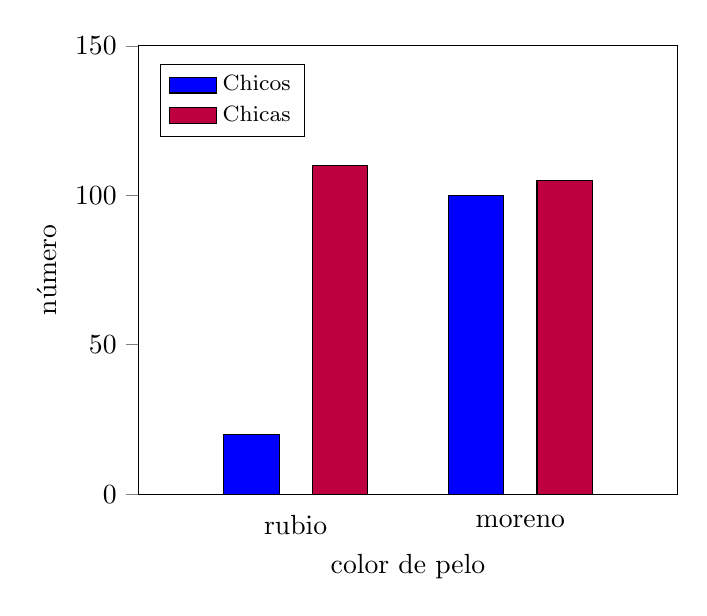
\begin{tikzpicture}
	\begin{axis}[
	    ybar=12pt,
	    ymin=0,ymax=150,
	    xtick=data,
	    enlarge x limits={abs=2cm},
	    symbolic x coords={rubio, moreno},
	    bar width = 20pt,
	    ylabel= número,
	    xlabel= color de pelo,
	        ytick align=outside,
	        ytick pos=left,
	        major x tick style = transparent,
	        legend style={at={(0.04,0.96)},anchor=north west, font=\footnotesize, legend cell align=left,},
	        ]
	    \addplot[ybar,fill=blue, area legend] coordinates {
	        (rubio,20)
	        (moreno,100)};
	    \addplot[ybar,fill=purple, area legend] coordinates {
	        (rubio,110)
	        (moreno,105)};
	 \legend{Chicos, Chicas}
	\end{axis}
\end{tikzpicture}
\caption{Gráfica barras.}
\end{figure}
\end{lstlisting}

El resultado es el siguiente:

\begin{figure}[ht]
\centering
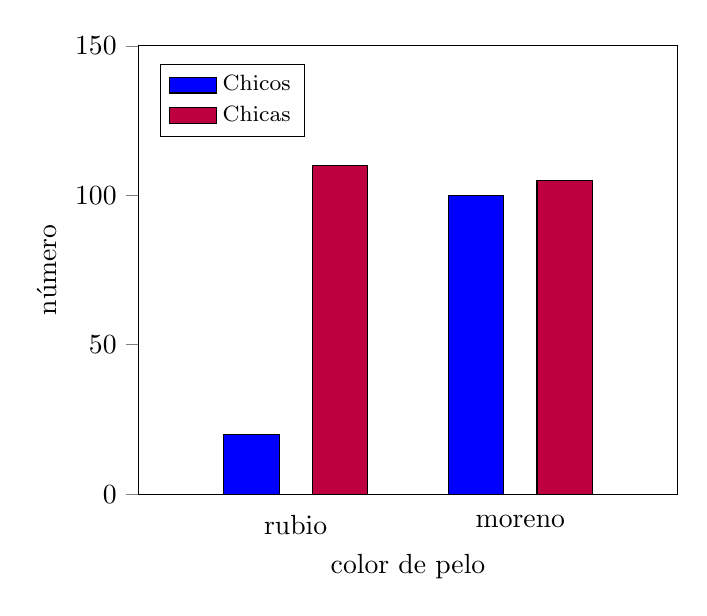
\begin{tikzpicture}
	\begin{axis}[
	    ybar=12pt,
	    ymin=0,ymax=150,
	    xtick=data,
	    enlarge x limits={abs=2cm},
	    symbolic x coords={rubio, moreno},
	    bar width = 20pt,
	    ylabel= número,
	    xlabel= color de pelo,
	        ytick align=outside,
	        ytick pos=left,
	        major x tick style = transparent,
	        legend style={at={(0.04,0.96)},anchor=north west, font=\footnotesize, legend cell align=left,},
	        ]
	    \addplot[ybar,fill=blue, area legend] coordinates {
	        (rubio,20)
	        (moreno,100)};
	    \addplot[ybar,fill=purple, area legend] coordinates {
	        (rubio,110)
	        (moreno,105)};
	 \legend{Chicos, Chicas}
	\end{axis}
\end{tikzpicture}
\caption{Gráfica barras.}
\end{figure}
\FloatBarrier

\subsection{Polar}
Un ejemplo de gráfica polar semicircular (ver archivo archivos/ejemplos/polarnorm.tex):

\begin{figure}[H]
    	\centering%
         {\scalefont{0.8}%
    \input{archivos/ejemplos/polarnorm}%
    }
    \caption{Directividad normalizada del altavoz (0 dBV en el eje).}\label{norma}
\end{figure}


\section{Importados de MATLAB}
\label{impmatlab}
Gracias a la herramienta \textit{matlab2tikz} (\url{https://es.mathworks.com/matlabcentral/fileexchange/22022-matlab2tikz-matlab2tikz}) se pueden exportar las gráficas de cualquier tipo de Matlab a latex.
Después de incluir los archivos de \textit{matlab2tikz} se debe escribir una llamada después de crear la figura tal que:

\begin{lstlisting}[style=Matlab-color,caption={Ejemplo de llamada a matlab2tikz}]
fig = plot(x,y);
matlab2tikz('figurehandle',fig,'NombreArchivo.tex','height','5cm','width','13.5cm','strict',true,'showHiddenStrings',true,'showInfo',false)
\end{lstlisting}

Y para utilizar el archivo generado por la función en este documento:
\begin{lstlisting}[style=Latex-color]
\begin{figure}[ht]
	\centering
	{\scalefont{0.8}\input{archivos/ejemplos/ParedFina} }
	\caption{Ejemplo de gráfica obtenida con matlab2tikz.}
\end{figure}
\end{lstlisting}

\begin{figure}[ht]
	\centering
	{\scalefont{0.8}\input{archivos/ejemplos/ParedFina} }
	\caption{Ejemplo de gráfica obtenida con matlab2tikz.}
\end{figure}
\FloatBarrier
Ejemplo de una gráfica 3D generada en Matlab y exportada por \textit{matlab2tikz}:
\begin{figure}[ht]
		\centering
		{\scalefont{0.8}\input{archivos/ejemplos/2D-3314hz} }
		\caption{Amplitud de la aceleración en el modo número 8.}
\end{figure}
\FloatBarrier

\section{Ejemplo avanzado}

El potencial del paquete \textit{Tikz} es muy alto, se pueden realizar muchísimas cosas. En la red se facilitan muchos ejemplos para poder ver el funcionamiento y aprender. Existen hilos donde la gente publica sus mejores diseños de \textit{Tikz} como en \url{https://tex.stackexchange.com/questions/158668/nice-scientific-pictures-show-off} o páginas donde facilitan muchas plantillas como \url{http://www.texample.net/tikz/examples/all/}.
\par Un ejemplo de lo que se puede llegar a conseguir es el siguiente:
% Vector Styles
\tikzset{
  load/.style   = {ultra thick,-latex},
  stress/.style = {-latex},
  dim/.style    = {latex-latex},
  axis/.style   = {-latex,black!55},
}

% Drawing View
\tikzset{dimetric2/.style={
  x={(0.935cm,-0.118cm)},
  y={(0.354cm, 0.312cm)},
  z={(0.000cm, 0.943cm)},
}}
\begin{figure}[ht]
\centering
  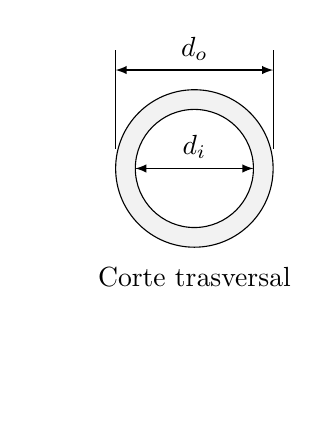
\begin{tikzpicture}
    \node (origin) at (0,0) {}; % shift relative baseline
    \coordinate (O) at (2,3);
    \draw[fill=gray!10] (O) circle (1);
    \draw[fill=white] (O) circle (0.75) node[below,yshift=-1.125cm] {Corte trasversal};
    \draw[dim] (O) ++(-0.75,0) -- ++(1.5,0) node[midway,above] {$d_i$};
    \draw[dim] (O) ++(-1,1.25) -- ++(2,0) node[midway,above] {$d_o$}; 
    \foreach \x in {-1,1} {
      \draw (O) ++(\x,0.25) -- ++(0,1.25);
    }
  \end{tikzpicture}
  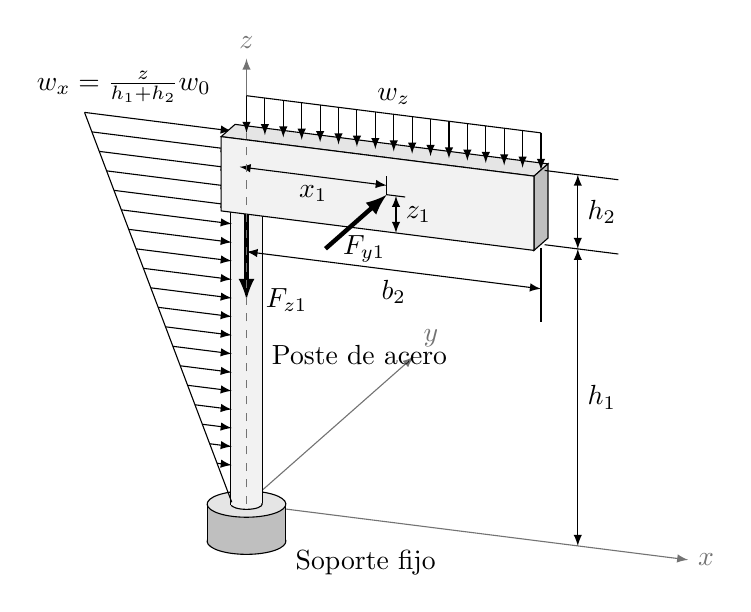
\begin{tikzpicture}[dimetric2]
        \coordinate (O) at (0,0,0);
        \draw[axis] (O) -- ++(6,0,0) node[right] {$x$};
        \draw[axis] (O) -- ++(0,6,0) node[above right] {$y$};
        \draw[axis] (O) -- ++(0,0,6) node[above] {$z$};
        \draw[fill=gray!50] (0,0,-0.5) circle (0.5); 
        \fill[fill=gray!50] (-0.46,-0.2,-0.5) -- (0.46,0.2,-0.5) -- (0.46,0.2,0) -- (-0.46,-0.2,0) -- cycle;
        \draw[fill=gray!20] (O) circle (0.5);
    \draw (0.46,0.2,-0.5) -- ++(0,0,0.5) node[below right,pos=0.0] {Soporte fijo};
    \draw (-0.46,-0.2,-0.5) -- ++(0,0,0.5);
    \draw[fill=gray!10] (O) circle (0.2);
    \fill[fill=gray!10] (-0.175,-0.1,0) -- (0.175,0.1,0) -- ++(0,0,4) -- (-0.175,-0.1,4) -- cycle;
    \draw (-0.175,-0.1,0) -- ++(0,0,4);
    \draw (0.175,0.1,0) -- ++(0,0,4) node[right,midway] {Poste de acero};
    \draw (4,0,3.95) -- ++(0,0,-1);
    \foreach \z in {0.5,0.75,...,5} {
      \draw[-latex] (-2*\z/5-0.2,0,\z) -- (-0.2,0,\z);
    }
    \draw[load] (0,0,4) -- ++(0,0,-1.25) node[right,xshift=0.1cm] {$F_{z1}$};
    \draw[fill=gray!20] (-0.25,-0.25,5) -- (4,-0.25,5) -- (4,+0.25,5) -- (-0.25,+0.25,5) -- cycle; 
    \draw[fill=gray!50] (+4.00,-0.25,4) -- (4,+0.25,4) -- (4,+0.25,5) -- (+4.00,-0.25,5) -- cycle; 
    \draw[fill=gray!10] (-0.25,-0.25,4) -- (4,-0.25,4) -- (4,-0.25,5) -- (-0.25,-0.25,5) -- cycle; 
    \draw (4.05,0,4) -- ++(1,0,0);
    \draw (4.05,0,5) -- ++(1,0,0);
    \draw[dim] (4.5,0,0) -- ++(0,0,4) node[midway,right] {$h_1$};
    \draw[dim] (4.5,0,4) -- ++(0,0,1) node[midway,right] {$h_2$};
    \draw[dim] (0,0,3.4) -- ++(4,0,0) node[midway,below] {$b_2$};
    \coordinate (P) at (2,-0.25,4.5);
    \draw (P) -- ++(0,0,0.25);
    \draw (P) -- ++(0.25,0,0);
    \draw[dim] (2.125,-0.25,4.5) -- ++(0,0,-0.5) node[midway,right] {$z_1$};
    \draw[dim] (2,-0.25,4.625) -- ++(-2,0,0) node[midway,below] {$x_1$};
    \draw[load] (2,-2.45,4.5) -- ++(0,2.2,0) node[pos=0.0,right,xshift=0.08cm] {$F_{y1}$};
    \draw[axis,dashed,-] (O) -- (0,0,5);
    \draw (0,0,5.5) -- ++(4,0,0) node[midway,above] {$w_{z}$};
    \foreach \x in {0,0.25,...,4} {
      \draw[-latex] (\x,0,5.5) -- ++(0,0,-0.5);
    }
    \draw (-0.2,0,0) -- ++(-2,0,5) node[above,xshift=0.5cm] {$w_{x}=\frac{z}{h_1+h_2} w_0$};
  \end{tikzpicture}
\caption{Señal realizada con Tikz, sin imágenes.}
\label{senyal}
\end{figure}
\FloatBarrier

